%----------------------------------------------------------
\subsection{Espacio de Colores}
Para extraer los objetos de la escena, el algoritmo simplifica los colores de cada imagen y agrupa los p\'ixeles en cl\'usteres de colores. \\

RGB es el espacio de colores mas com\'un, este est\'a compuesto de tres canales (Rojo, verde y azul).Sin embargo, el principal problema de este espacio de colores es que la información sobre la "pigmentaci\'on" se encuentra en los tres canales.\\

Para solventar ese problema, se usa en este proyecto el espacio de colores HSV (Hue, Saturation and Value). En este, la información sobre el color se encuentra en un único canal, por lo que es menos sensible a los cambios y las limitaciones entre un color y otro son planos en vez de superficies. \\

% HSV vs RGB figure
\begin{figure}[h]
	\centering
	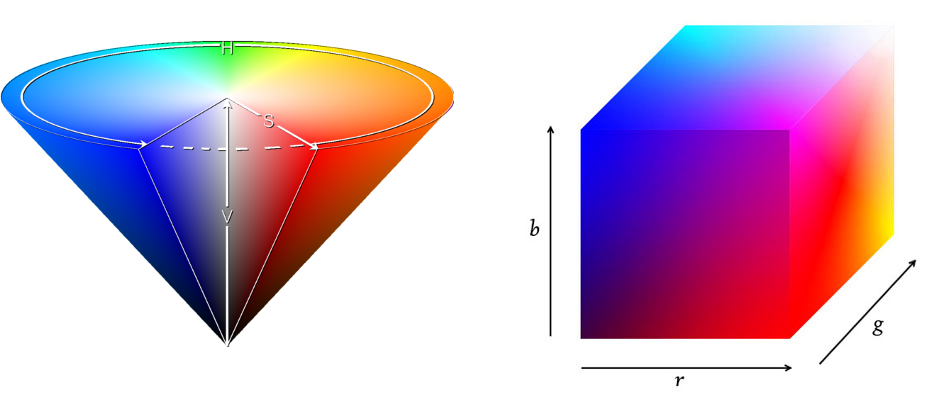
\includegraphics[width=0.75\textwidth,natwidth=944,natheight=400]{../Images/c2/HSV_vs_RGB.png}
	\caption{Espacios de colores HSV y RGB}
	\label{fig:HSV_vs_RGB}
\end{figure}

%----------------------------------------------------------
\subsection{Transformaci\'on de pixeles}
En este apartado se describe c\'omo es transformado cada p\'ixel para pasar del color inicial a uno de los colores de los cl\'usteres. Esto se lleva a cabo aplicando una serie de límites a los canales del espacio de colores \\

\begin{figure}[h]
	\centering
	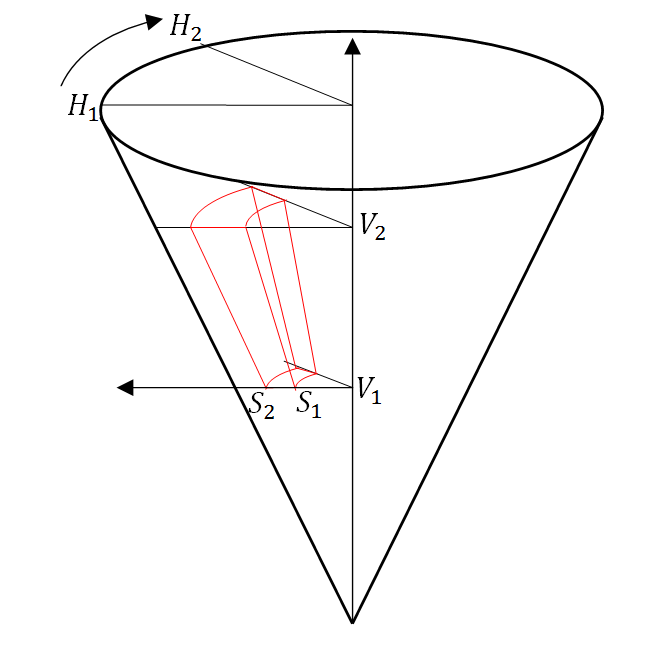
\includegraphics[width=0.5\textwidth,natwidth=659,natheight=659]{../Images/c2/DividingSubSpace.png}
	\caption{Divisi\'on del espacio de color HSV}
	\label{fig:DividingSubSpace}
\end{figure}

Una de las claves para la disminución del tiempo de computaci\'on del algoritmo es la sustitución de las condiciones $if...else...$ por in-direccionamientos de memoria y comparaciones $bitwise$. Estas son mucho m\'as r\'apidas y eficientes \cite{JamesBruce_CMU_SEG}. \\

\begin{equation}
\begin{split}
pixel\_col = H\_Range[h] \& \\
S\_Range[s] \& \\
V\_Range[v] 
\end{split}
\end{equation}
	

Para mostrar el proceso, consideramos el siguiente ejemplo. Si dividimos cada canal del espacio en diez bloques $(n_H = 10, n_S = 10$ y $n_V = 10)$ podemos definir de la siguiente forma (Indicando 1 cuando el negro pertenece a ese rango y 0 si no pertenece a ese rango)

{\centering
\[HRange[10] = \{1, 1, 1, 1, 1, 1, 1, 1, 1, 1\}\]
\[SRange[10] = \{1, 1, 1, 1, 1, 1, 1, 1, 1, 1\}\]
\[VRange[10] = \{1, 1, 1, 0, 0, 0, 0, 0, 0, 0\}\]
} 

Para comprobar si el siguiente color de p\'ixel:  $(3, 5, 1)$, pertenece al negro solo hay que evaluar la siguiente expresi\'on:

\[ pixel\_col = HRange[3] \& SRange[5] \& VRange[1] = 1 \& 1 \& 1 = 1 \]


El siguiente punto importante es que esto permite evaluar la pertenencia a muchas clases de colores de forma simultánea. Si definimos por ejemplo el azul como lo siguiente:

{\centering
\[HRange[10] = \{0, 0, 0, 0, 1, 1, 1, 0, 0, 0\}\]
\[SRange[10] = \{0, 0, 0, 0, 1, 1, 1, 1, 1, 1\}\]
\[VRange[10] = \{0, 0, 0, 1, 1, 1, 1, 1, 1, 1\}\]
}

Podremos agrupar ambos tipos así:

{\centering
\[HRange[10] = \{01, 01, 01, 01, 11, 11, 11, 01, 01, 01\}\]
\[SRange[10] = \{01, 01, 01, 01, 11, 11, 11, 11, 11, 11\}\]
\[VRange[10] = \{01, 01, 01, 10, 10, 10, 10, 10, 10, 10\}\] 
} 

Gracias a que la operaci\'on bitwise se realiza bit a bit, el color $(3,5,1)$ se puede evaluar como: 

\[pixel\_col = HRange[3] \& SRange[5] \& VRange[1] = 01 \& 11 \& 01 = 01\]

Resultando que pertenece al color negro.

En particular, en el algoritmo usamos arrays de bytes de tamaño 36, lo que significa que diferenciamos 8 colores con una resoluci\'on de $1/36$. \\

Las siguientes imágenes muestran el resultado del algoritmo con la conocida imagen \textit{Head Scene}  de la universidad de Tsukuba \ref{fig:head_scene_tsukuba_ori} \ref{fig:head_scene_tsukuba_seg}. \\


\begin{figure}[hbp]
	\centering
	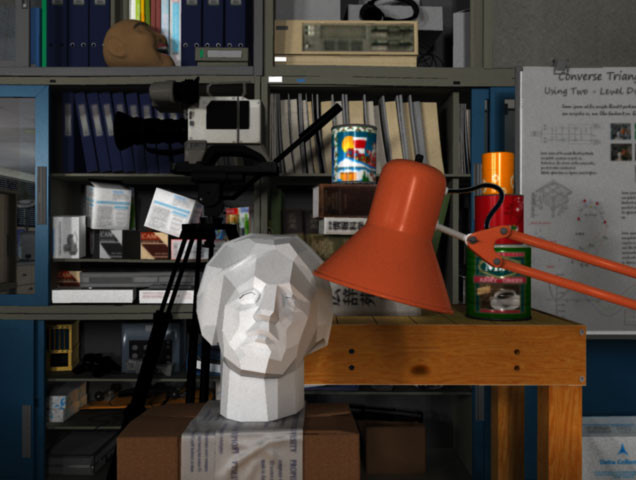
\includegraphics[width=0.4\linewidth]{../Images/c2/head_scene_tsukuba_ori}
	\caption{Imagen original de $Head Scene$}
	\label{fig:head_scene_tsukuba_ori}
\end{figure}

\begin{figure}[htp]
	\centering
	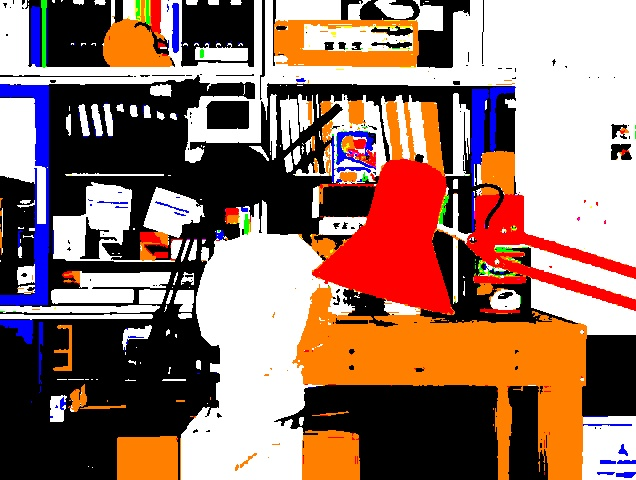
\includegraphics[width=0.4\linewidth]{../Images/c2/head_scene_tsukuba_seg}
	\caption{Imagen segmentada de $Head Scene$}
	\label{fig:head_scene_tsukuba_seg}
\end{figure}



%\begin{figure}[h]
%	\centering
%	\begin{subfigure}{0.47\linewidth}
%		\centering
%		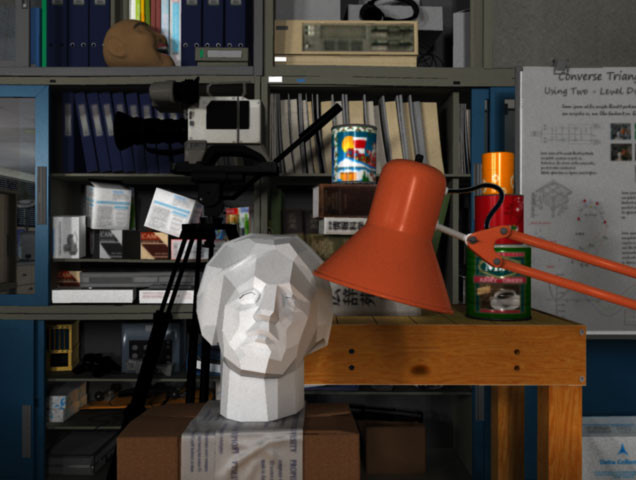
\includegraphics[width=\linewidth]{../Images/c2/head_scene_tsukuba_ori}
%		\caption{Original image of the Head Scene}
%		\label{fig:head_scene_tsukuba_ori}
%	\end{subfigure}
%	~
%	\begin{subfigure}{0.47\linewidth}
%		\centering
%		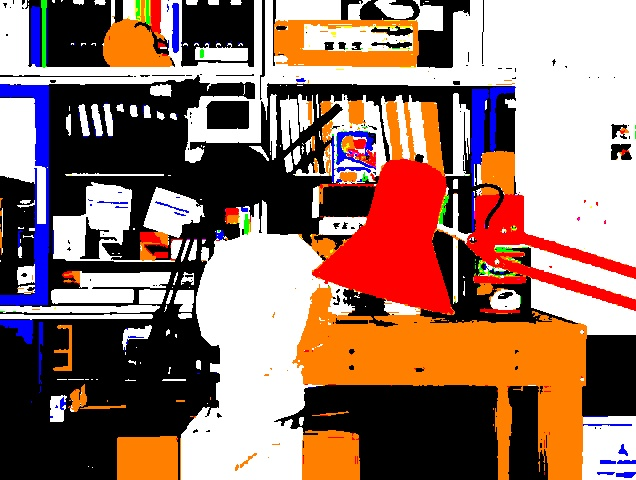
\includegraphics[width=\linewidth]{../Images/c2/head_scene_tsukuba_seg}
%		\caption{Segmented image of the Head Scene}
%		\label{fig:head_scene_tsukuba_seg}
%	\end{subfigure}
%	\caption{Head Scene, University of Tsukuba}
%	\label{fig:Head_Scene}
%\end{figure}



%----------------------------------------------------------
\subsection{Run-length encoding}
La compresi\'on RLE o $Run-length encoding$ es un m\'etodo simple de compresión de datos donde cada tira de datos del mismo tipo es comprimida por una pareja de $valor$ y $cantidad$. Por ejemplo, la siguiente $tira$: \\

\textit{WWWWWWWBBBBBBBBBCCCCCCWWWWWWWWWWWWWWWW} \\

Codificada seria la siguiente: \\
\textit{W7B9C6W16}

En este documento RLE se usa para reducir el tama\~no de la imagen, permitiendo iterar r\'apidamente en cada iteraci\'n. \\

Este tipo de compresión es muy útil en las imágenes que tienen colores homogéneos, sin embargo puede aumentar el tama\~no de la misma si los p\'ixeles tienen demasiado ruido: \\

\begin{enumerate}
	\item Homog\'eneo: \textit{WWWWWWWWWWWWWWWWWWWW $\Rightarrow$ W20} \\
	\item Heterog\'eneo: \textit{WAWAWAWAWA $\Rightarrow$ W1A1W1A1W1A1W1A1} \\
\end{enumerate}

%----------------------------------------------------------
\subsection{Agrupaci\'on de p\'ixeles. Creaci\'on del objeto}

Una vez comprimida la imagen es necesario conectar las regiones de la imagen para crear los objetos \ref{fig:RLE1}. Esto se hace en dos etapas. La primera se buscan las relaciones entre una fila y su consecutiva, tal que se unen si son del mismo color \ref{fig:RLE2}. Una vez exploradas todas las l\'ineas \ref{fig:RLE3}, la segunda etápa busca los objetos divididos y los agrupa \ref{fig:RLE4}. En esta \'ultima etapa los se almacena la información dentro de la $clase objeto$, que contiene la información de los RLE.

\begin{figure}
	\centering
	\begin{subfigure}{\linewidth}
		\centering
		\begin{subfigure}{0.4\linewidth}
			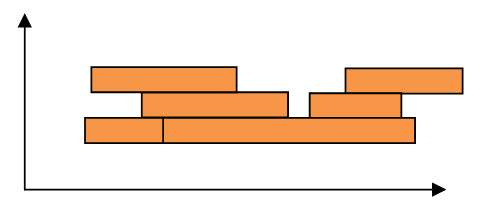
\includegraphics[width=\linewidth]{../Images/c2/RLE1}
			\caption{Conjuntos no unidos}
			\label{fig:RLE1}
		\end{subfigure}
		%--------------------------------------------------------------------
		\begin{subfigure}{0.4\linewidth}
			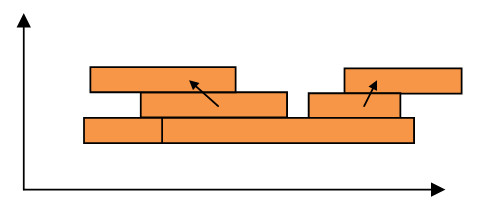
\includegraphics[width=\linewidth]{../Images/c2/RLE2}
			\caption{Recorrido vertical}
			\label{fig:RLE2}
		\end{subfigure}
	\end{subfigure}
	~
	\begin{subfigure}{\linewidth}
		\centering
   		\begin{subfigure}{0.4\linewidth}
   			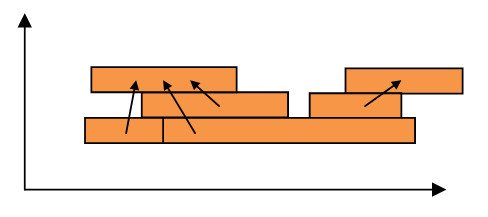
\includegraphics[width=\linewidth]{../Images/c2/RLE3}
   			\caption{Conjuntos unidos}
   			\label{fig:RLE3}
   		\end{subfigure}
   		%--------------------------------------------------------------------
   		\begin{subfigure}{0.4\linewidth}
   			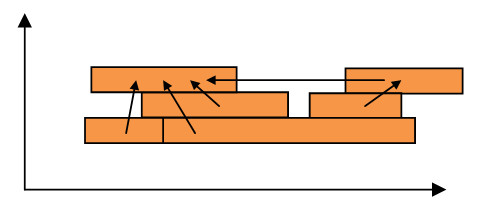
\includegraphics[width=\linewidth]{../Images/c2/RLE4}
   			\caption{B\'usqueda de objetos divididos}
   			\label{fig:RLE4}
   		\end{subfigure}
	\end{subfigure}
	\caption{Creaci\'on de objetos desde los RLE}
\end{figure}
